\chapter{Enclosure and Convex Distance}
\label{ch:enclosure_convex_distance}

\section{Welzl's Algorithm}
\label{sec:welzls_algorithm}

\subsection{Overview}
Welzl's algorithm\index{Welzl's algorithm} is a randomized algorithm for finding the smallest enclosing circle (the minimum-area circle that contains all points in a set). Originally described by Emo Welzl in 1991~\cite{welzl1991}, it is a brilliant application of the linear programming paradigm to a geometric problem. The algorithm builds on earlier linear-time results for fixed-dimension linear programming by Megiddo~\cite{megiddo1983}. It achieves an expected $O(n)$ time complexity, making it highly efficient for point sets in 2D.

\subsection{Definitions}

\begin{definition}[Smallest Enclosing Circle]\label{def:sec}
The \textbf{smallest enclosing circle (SEC)}\index{smallest enclosing circle} of a point set $P \subset \mathbb{R}^2$ is the unique circle of minimum radius that contains every point of $P$. The SEC is also called the \emph{minimum covering circle} or \emph{minidisk}.
\end{definition}

\begin{definition}[Support Points]\label{def:support_points}
The \textbf{support points}\index{support points} of the SEC are the points of $P$ that lie on the boundary of the SEC. The SEC is uniquely determined by at most three support points: a single point (the center), two points (the circle having them as diameter), or three non-collinear points (the circumcircle).
\end{definition}

\subsection{Theory}
The algorithm is based on a recursive reduction of the point set. The key insight is that if a new point $P_i$ is already inside the SEC of the previous $i-1$ points, then the SEC remains the same. If $P_i$ is outside, it MUST lie on the boundary of the new SEC. This allows us to recursively solve the problem with $P_i$ fixed as a ``boundary point.''

The recursion continues until we have a set of 0, 1, 2, or 3 points that must lie on the boundary. These ``fixed'' points uniquely define the circle (0: none, 1: point as center, 2: segment as diameter, 3: circumcircle).

\begin{theorem}[Expected Linear Time]\label{thm:welzl_linear}
Welzl's algorithm computes the smallest enclosing circle of $n$ points in $\mathbb{R}^2$ in expected $O(n)$ time.
\end{theorem}

\begin{proof}
The proof uses a backwards analysis argument. Fix a random permutation $\pi$ of the $n$ points. Consider the moment when the algorithm first inserts a point $p_{\pi(i)}$ onto the boundary (i.e., the recursion rejects the current disk and adds $p_{\pi(i)}$ to $R$). By backwards analysis, conditioning on this event, $p_{\pi(i)}$ is equally likely to be any of the $i$ points seen so far. The expected number of boundary insertions across all $n$ points is $\sum_{i=1}^{n} \frac{3}{i} = O(\log n)$ (since at most 3 points are ever on the boundary and each insertion reduces the remaining budget by 1). The total work is therefore $O(n + \log n) = O(n)$. See~\cite{welzl1991} and Megiddo~\cite{megiddo1983} for the full analysis.
\end{proof}

\begin{figure}[htbp]
\centering
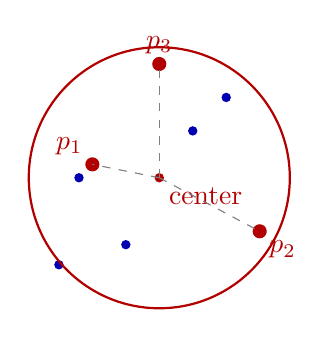
\begin{tikzpicture}[scale=0.85]
  \foreach \x/\y in {1/2, 2/3.5, 3.5/1, 0.5/0.5, 3/3, 1.5/0.8, 2.5/2.5, 0.8/1.8} {
    \fill[blue!70!black] (\x,\y) circle (2pt);
  }
  \fill[red!70!black] (1,2) circle (3pt) node[above left] {$p_1$};
  \fill[red!70!black] (3.5,1) circle (3pt) node[below right] {$p_2$};
  \fill[red!70!black] (2,3.5) circle (3pt) node[above] {$p_3$};
  \draw[thick,red!70!black] (2,1.8) circle (1.95);
  \fill[red!70!black] (2,1.8) circle (2pt) node[below right] {center};
  \draw[gray,dashed] (2,1.8)--(1,2);
  \draw[gray,dashed] (2,1.8)--(3.5,1);
  \draw[gray,dashed] (2,1.8)--(2,3.5);
\end{tikzpicture}
\caption{Welzl's algorithm: the smallest enclosing circle is defined by at most 3 support points (red).}
\label{fig:welzl}
\end{figure}


\begin{example}[Welzl Recursion Trace]\label{ex:welzl}
Consider points $P = \{(0,0), (4,0), (2,3), (2,1)\}$ processed in order:
\begin{enumerate}
    \item Recurse with $R = \{\}$: pop $(2,1)$, compute SEC of remaining 3 points. The SEC of $\{(0,0),(4,0),(2,3)\}$ is the circumcircle: center $(2, 0.833)$, radius $\approx 2.404$.
    \item Check $(2,1)$: distance from center is $\approx 0.167 < 2.404$---inside! Return this SEC.
\end{enumerate}
The algorithm finishes in one pass because $(2,1)$ happens to be interior to the circumcircle of the other three.
\end{example}

\subsection{Pseudocode}
\begin{algorithm}[ht]
\label{alg:welzl}
\begin{algorithmic}[1]
\Function{Welzl}{$P$, $R$ = []}
    \If{$|P| = 0$ \textbf{or} $|R| = 3$}
        \State \Return \Call{CircleFromBoundary}{$R$}
    \EndIf
    \State $p \gets P.\text{pop}()$
    \State $D \gets \text{Welzl}(P.\text{copy}(),\; R)$
    \If{$p$ is in $D$}
        \State \Return $D$
    \EndIf
    \State \Return \text{Welzl}($P.\text{copy}()$, $R + [p]$)
\EndFunction
\Statex
\Comment{To start:}
\State $\text{random.shuffle}(\text{points})$
\State $\text{SEC} \gets \text{Welzl}(\text{points})$
\end{algorithmic}
\end{algorithm}

\subsection{Parameter Selection}
\begin{itemize}
    \item \textbf{Randomization}: Shuffling the input points at the beginning is crucial. Without randomization, structured input (like points on a line) can cause $O(n^2)$ worst-case performance.
    \item \textbf{Numerical Precision}: Circumcircle calculations for 3 points can be sensitive to collinearity. An epsilon should be used to check if 3 points are nearly on a line.
\end{itemize}

\subsection{Complexity}
\begin{itemize}
    \item \textbf{Time Complexity}: $O(n)$ expected. Although the recursion depth is $n$, the probability that a point falls outside the current circle decreases rapidly, leading to the $O(n)$ bound.
    \item \textbf{Space Complexity}: $O(n)$ for the recursion stack and the copies of the point set.
\end{itemize}

\subsection{Usages}
\begin{itemize}
    \item \textbf{Collision Detection}: Generating a bounding sphere for an object as a fast first-pass check~\cite{ericson2004}.
    \item \textbf{Facility Location}: Finding the center for a new resource (e.g., a cell tower) to cover all clients with minimum range.
    \item \textbf{Cluster Analysis}: Determining the spatial extent of a group of points.
    \item \textbf{Camera Control}: Finding the minimum zoom/pan to keep all characters in a scene visible.
\end{itemize}

\subsection{Testing Methods and Edge Cases}
\begin{itemize}
    \item \textbf{Collinear Points}: The SEC should have its diameter equal to the distance between the two furthest points.
    \item \textbf{Duplicate Points}: Handled naturally by the inclusion check.
    \item \textbf{Small Sets}: Verify with 0, 1, and 2 points.
    \item \textbf{Symmetry}: Regular polygons should result in a circle centered at the polygon's centroid.
    \item \textbf{Redundant Points}: Verify that a million points inside a circle don't change the SEC defined by 3 points on the boundary.
\end{itemize}

\subsection{References}
\begin{itemize}
    \item Welzl, E. (1991). ``Smallest enclosing disks (balls and ellipsoids)''. Lecture Notes in Computer Science.
    \item Megiddo, N. (1983). ``Linear-time algorithms for linear programming in $\mathbb{R}^3$ and related problems''. SIAM Journal on Computing.
    \item Wikipedia: \href{https://en.wikipedia.org/wiki/Smallest-circle_problem}{Smallest-circle problem}
\end{itemize}

\section{Convex Polygon Distance}
\label{sec:convex_polygon_distance}

\subsection{Overview}
The convex polygon distance problem involves finding the minimum Euclidean distance between two non-intersecting convex polygons $P$ and $Q$. This is a fundamental operation in collision detection and motion planning. While a naive $O(n \cdot m)$ approach checks all pairs of edges, more efficient algorithms leverage the convexity of the shapes to achieve $O(n + m)$ or even $O(\log n + \log m)$ performance. The rotating calipers approach was popularized by Toussaint~\cite{toussaint1983}, and the GJK algorithm was introduced by Gilbert, Johnson, and Keerthi~\cite{gilbert1988}. Edelsbrunner~\cite{edelsbrunner1985} provides further complexity bounds.

\subsection{Definitions}

\begin{definition}[Euclidean Distance between Polygons]\label{def:euclidean_poly_dist}
The \textbf{Euclidean distance}\index{Euclidean distance} between two polygons $P$ and $Q$ is
\[
\operatorname{dist}(P, Q) = \min_{p \in P,\; q \in Q} \|p - q\|_2.
\]
For non-intersecting convex polygons, this minimum is achieved between two vertices or a vertex and an edge.
\end{definition}

\begin{definition}[Separating Axis]\label{def:separating_axis}
A \textbf{separating axis}\index{separating axis} is a line $\ell$ such that the orthogonal projections of two convex shapes $P$ and $Q$ onto $\ell$ do not overlap. By the separating axis theorem, two convex shapes do not intersect if and only if a separating axis exists.
\end{definition}

\begin{definition}[Minkowski Difference]\label{def:minkowski_difference}
The \textbf{Minkowski difference}\index{Minkowski difference} of two sets $P, Q \subset \mathbb{R}^2$ is
\[
P \ominus Q = \{p - q \mid p \in P,\; q \in Q\}.
\]
For convex polygons with $n$ and $m$ vertices, $P \ominus Q$ is a convex polygon with at most $n + m$ vertices. The distance $\operatorname{dist}(P,Q)$ equals the distance from the origin to $P \ominus Q$.
\end{definition}

\begin{definition}[GJK Algorithm]\label{def:gjk}
The \textbf{Gilbert--Johnson--Keerthi (GJK) algorithm}\index{GJK algorithm} computes the distance between two convex shapes by iteratively constructing a simplex inside the Minkowski difference $P \ominus Q$ that converges toward the origin. If the origin lies inside $P \ominus Q$, the shapes intersect.
\end{definition}

\subsection{Theory}
The most common approach for linear-time distance calculation is based on the \textbf{Rotating Calipers}\index{rotating calipers} method.
\begin{enumerate}
    \item Find the pair of points (one on each polygon) that minimize the distance. For non-intersecting convex polygons, this minimum distance occurs between two vertices, or a vertex and an edge.
    \item Use the rotating calipers technique to ``crawl'' around both polygons simultaneously. Because the polygons are convex, the distance function is unimodal along the boundary, allowing us to find the global minimum in a single pass.
\end{enumerate}

Another powerful approach is the \textbf{GJK Algorithm}:
\begin{enumerate}
    \item Compute the \textbf{Minkowski Difference} $D = P \ominus Q$.
    \item The distance between $P$ and $Q$ is the distance from the origin $(0,0)$ to the set~$D$.
    \item GJK iteratively builds a simplex inside $D$ that gets closer and closer to the origin.
\end{enumerate}

\begin{theorem}[Convex Distance Lower Bound]\label{thm:convex_dist}
For two convex polygons $P$ with $n$ vertices and $Q$ with $m$ vertices (both in convex position), the minimum Euclidean distance can be computed in $O(n + m)$ time using rotating calipers, and in $O(\log n + \log m)$ time using binary search if the polygons have been preprocessed.
\end{theorem}

\begin{proof}
The $O(n + m)$ bound follows from the rotating calipers observation: at each step, at least one caliper advances to the next vertex, and the total number of advances is at most $n + m$. The distance between the two caliper positions is evaluated at each step, and the minimum is returned. The $O(\log n + \log m)$ bound follows from the fact that for each edge of one polygon, the distance to the other polygon is a unimodal function along its boundary, which can be minimized by binary search.
\end{proof}

\subsection{Pseudocode}

\subsubsection*{Rotating Calipers for Distance}
\begin{algorithm}[ht]
\label{alg:convex_distance}
\begin{algorithmic}[1]
\Function{ConvexDistance}{$P$, $Q$}
    \State $i \gets \text{index\_of\_min\_y}(P)$
    \State $j \gets \text{index\_of\_max\_y}(Q)$
    \State $\text{min\_dist} \gets \infty$
    \For{$\_ \text{ in range}(|P| + |Q|)$}
        \State $d \gets \text{Distance}(P[i],\; Q[j])$
        \State $\text{min\_dist} \gets \min(\text{min\_dist},\; d)$
        \State $\text{angle\_P} \gets \text{AngleOfEdge}(P,\; i)$
        \State $\text{angle\_Q} \gets \text{AngleOfEdge}(Q,\; j)$
        \If{$\text{angle\_P} < \text{angle\_Q}$}
            \State $i \gets (i + 1) \bmod |P|$
        \Else
            \State $j \gets (j + 1) \bmod |Q|$
        \EndIf
    \EndFor
    \State \Return $\text{min\_dist}$
\EndFunction
\end{algorithmic}
\end{algorithm}

\begin{example}[Rotating Calipers Walkthrough]\label{ex:rotating_calipers}
Consider $P = \{(0,0), (3,0), (3,2), (0,2)\}$ (a $3 \times 2$ rectangle) and $Q = \{(5,1), (7,1), (7,3), (5,3)\}$ (a $2 \times 2$ rectangle). Both are CCW.
\begin{enumerate}
    \item Start: $i = $ index of min $y$ in $P = 0$ (point $(0,0)$), $j = $ index of max $y$ in $Q = 2$ (point $(7,3)$).
    \item Distance from $(0,0)$ to $(7,3)$: $\sqrt{49+9} = \sqrt{58} \approx 7.62$. Advance $i$ (edge $P[0] \to P[1]$ has angle $0^\circ$, smaller than $Q$'s edge).
    \item Distance from $(3,0)$ to $(7,3)$: $\sqrt{16+9} = 5.0$. Advance $j$.
    \item Continue until both calipers complete a full cycle. The minimum distance is $2.0$ (from edge $x=3$ of $P$ to edge $x=5$ of $Q$).
\end{enumerate}
\end{example}

\subsection{Parameter Selection}
\begin{itemize}
    \item \textbf{Polygon Orientation}: Polygons must be consistently oriented (e.g., both CCW).
    \item \textbf{Initial Points}: Starting at extreme points ensures the calipers are correctly synchronized.
\end{itemize}

\subsection{Complexity}
\begin{itemize}
    \item \textbf{Time Complexity}: $O(n + m)$ using rotating calipers or GJK. Binary search methods can achieve $O(\log n + \log m)$ for preprocessed polygons.
    \item \textbf{Space Complexity}: $O(1)$ auxiliary space if the polygons are already stored.
\end{itemize}

\subsection{Usages}
\begin{itemize}
    \item \textbf{Collision Avoidance}\index{collision detection}: Maintaining a ``safety buffer'' between a robot and obstacles.
    \item \textbf{Physics Simulation}: Calculating the time of impact or the depth of penetration.
    \item \textbf{Tolerance Analysis}: Determining if two mechanical parts will fit together with a required clearance.
    \item \textbf{UI Layout}: Calculating the spacing between complex geometric buttons or containers.
\end{itemize}

\subsection{Testing Methods and Edge Cases}
\begin{itemize}
    \item \textbf{Intersecting Polygons}: The distance should be 0. (GJK handles this by detecting that the origin is inside the Minkowski difference).
    \item \textbf{Parallel Edges}: The minimum distance might be achieved along an entire segment.
    \item \textbf{Points and Lines}: Test with ``polygons'' that are actually single points or line segments.
    \item \textbf{Very Thin Polygons}: Ensure numerical stability for nearly collinear vertices.
    \item \textbf{Vast Scales}: Precision check for polygons that are very far apart.
\end{itemize}

\subsection{References}
\begin{itemize}
    \item Toussaint, G.~T. (1983). ``Solving geometric problems with the rotating calipers''. Proceedings of MELECON '83.
    \item Gilbert, E.~G., Johnson, D.~W., \& Keerthi, S.~S. (1988). ``A fast procedure for computing the distance between complex objects in three-dimensional space''. IEEE Journal on Robotics and Automation.
    \item Edelsbrunner, H. (1985). ``Computing the extreme distances between two convex polygons''. Journal of Algorithms.
    \item Wikipedia: \href{https://en.wikipedia.org/wiki/Gilbert\%E2\%80\%93Johnson\%E2\%80\%93Keerthi_distance_algorithm}{Gilbert--Johnson--Keerthi distance algorithm}
\end{itemize}
